\section{Case Study Details}


\begin{figure}[t]
    \centering
    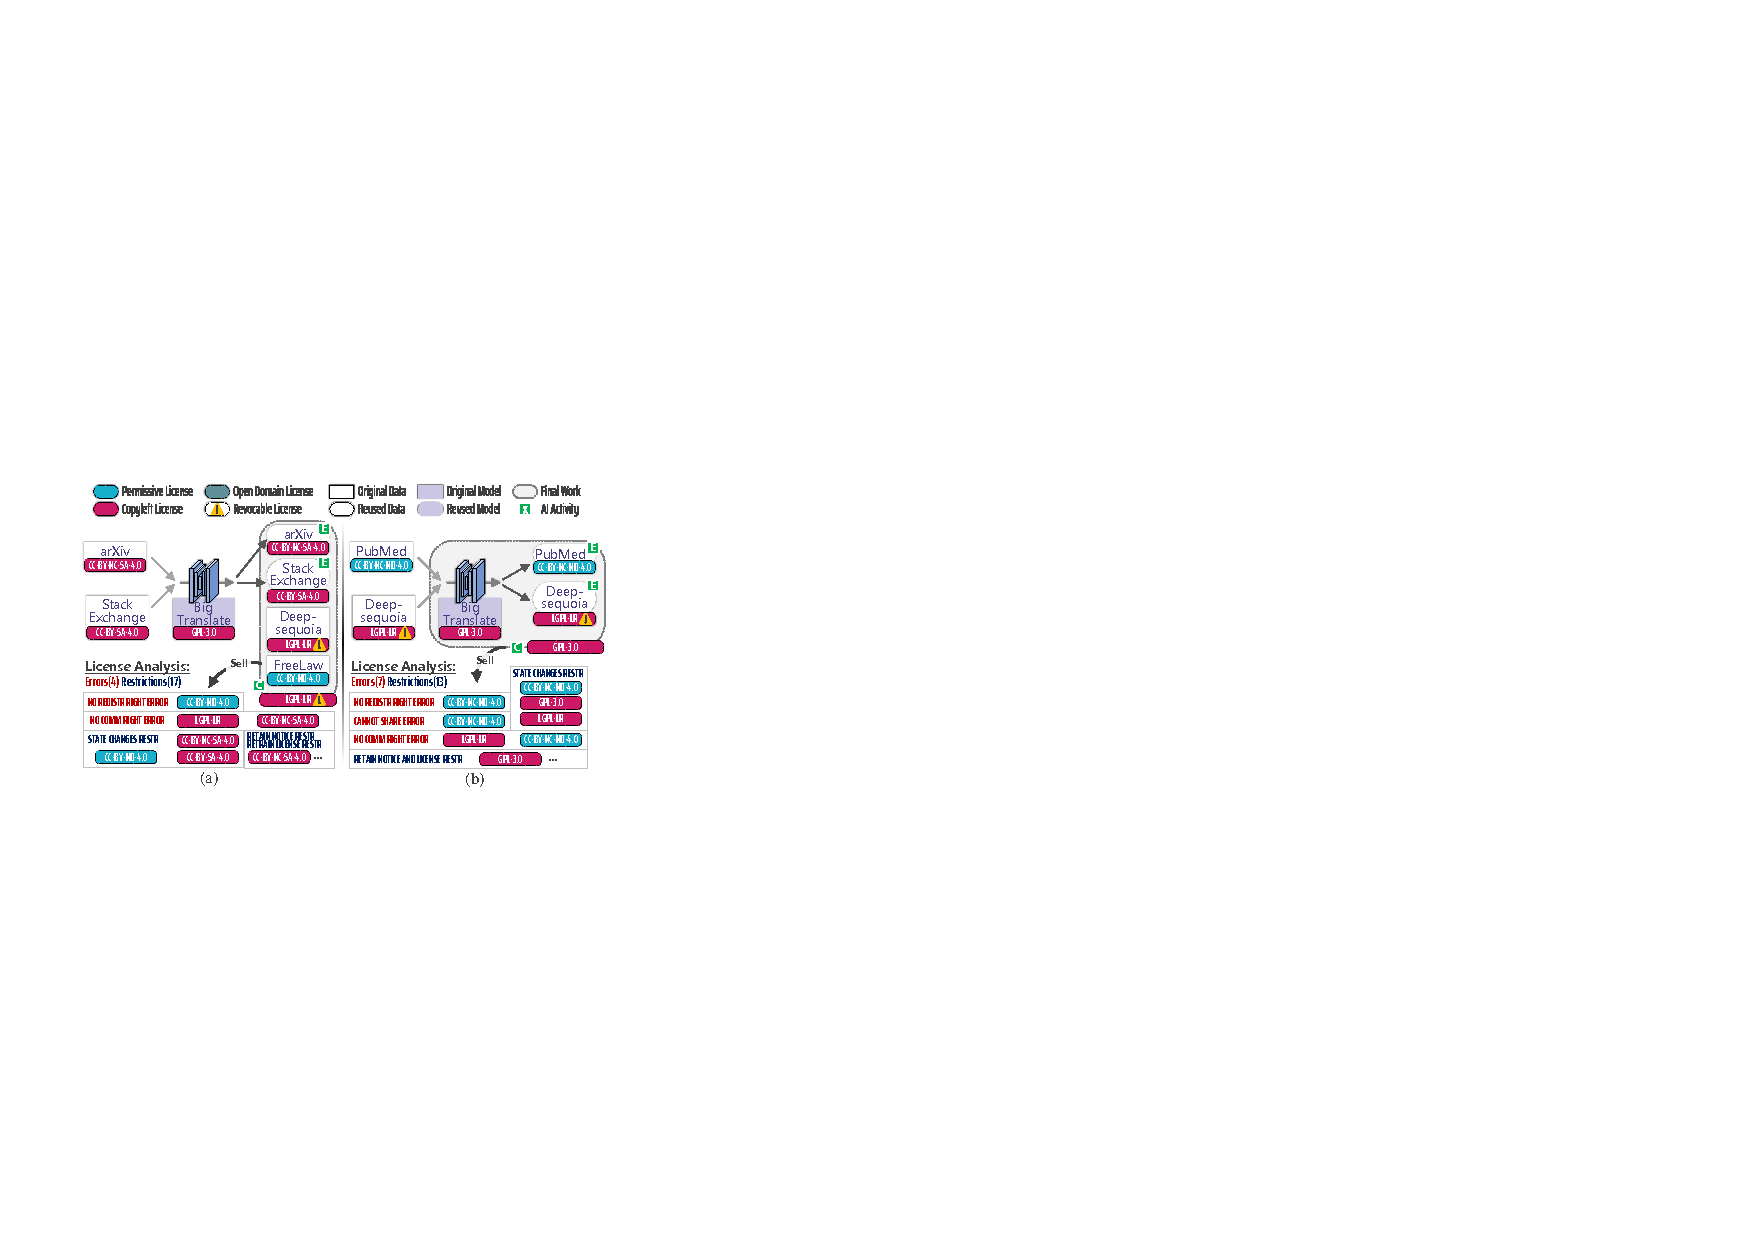
\includegraphics[width=\linewidth]{fig/case1.pdf}
    \caption{Case Study \Romannum{1}: Combination of Corpus. (a) LGPL-LR proliferation, CC collection; (b) LGPL-LR no linguistic resource, CC No redistribution.}
    \Description{}
    \label{fig:case1}
\end{figure}

\begin{figure}[t]
    \centering
    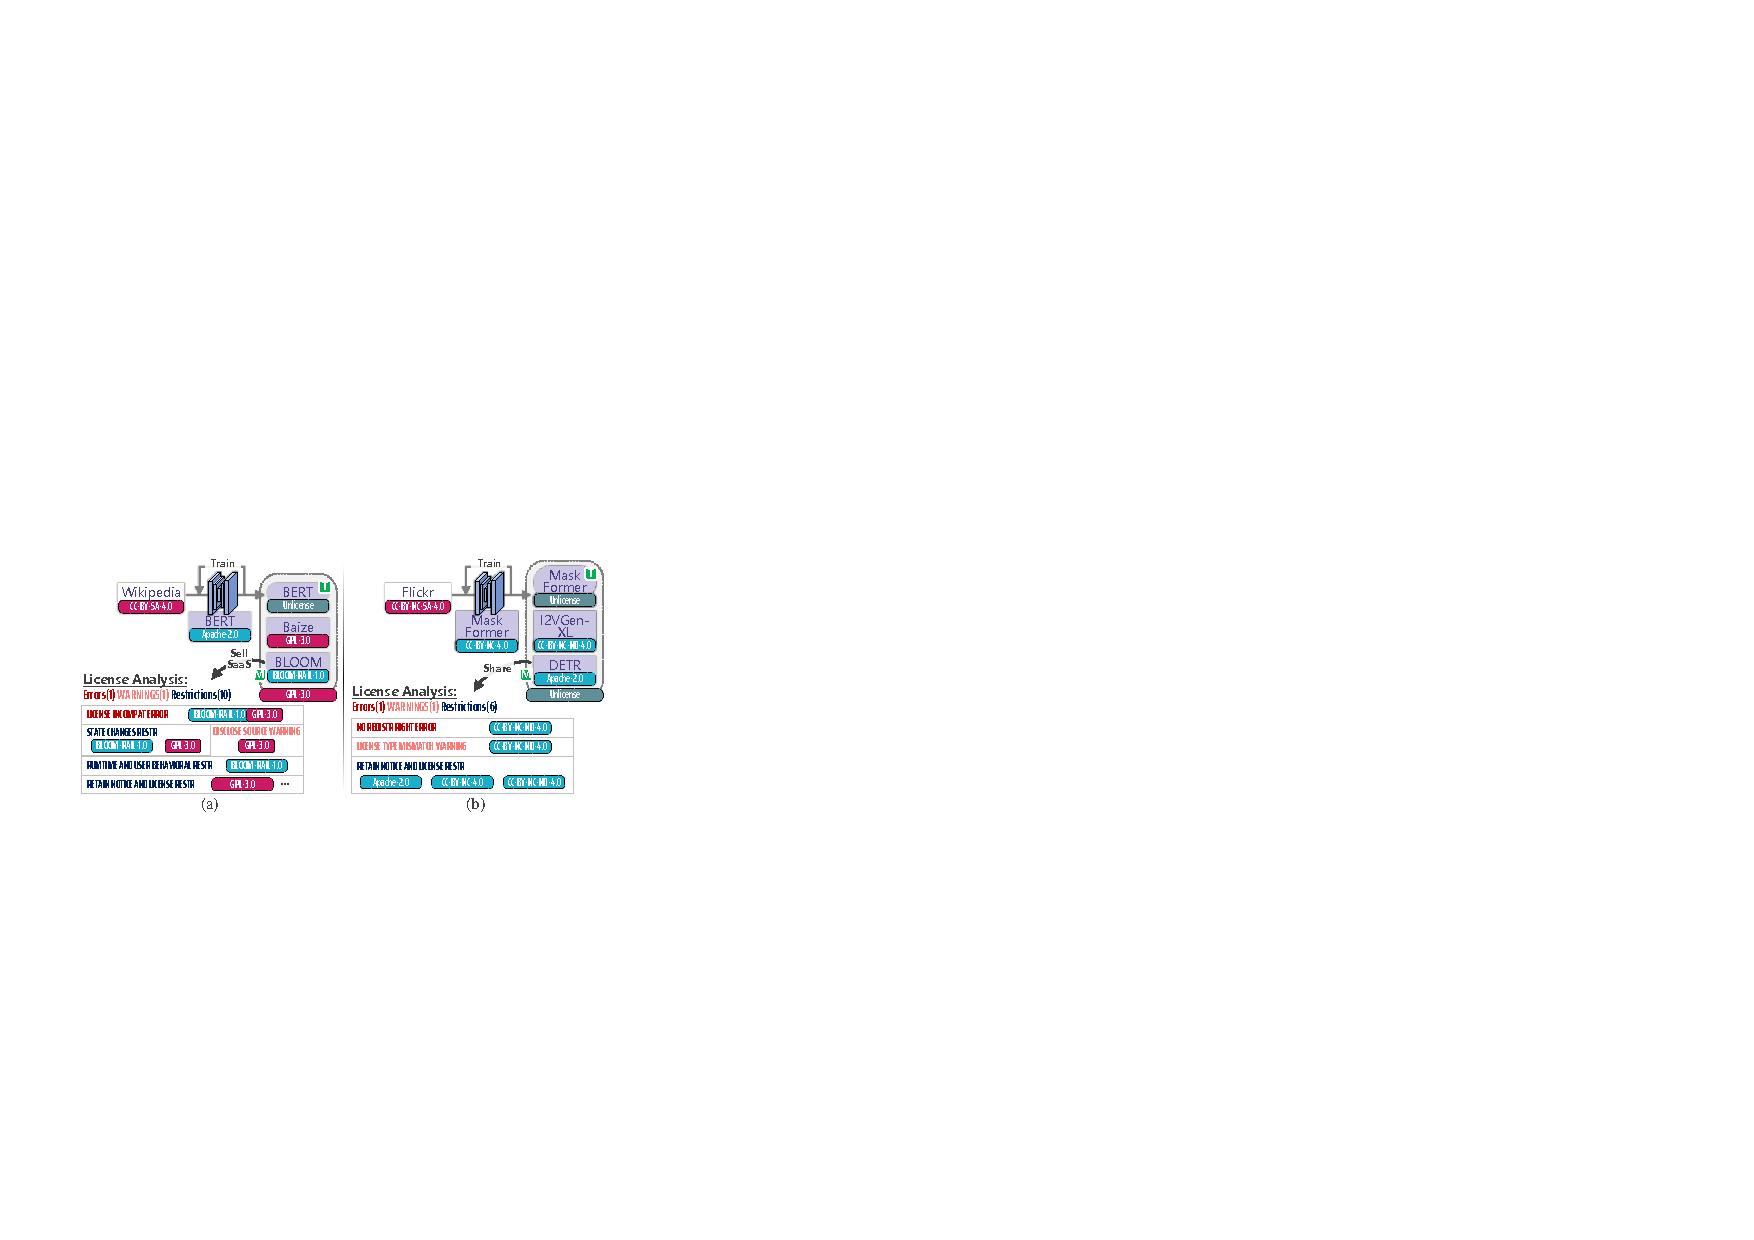
\includegraphics[width=\linewidth]{fig/case2.pdf}
    \caption{Case Study \Romannum{2}: Mixture of Experts. (a) BLOOM-RAIL, binary of GPL; (b) Unlicense, CC-BY-NC no distribute derivative. GPL Automatic Licensing of Downstream Recipients}
    \Description{}
    \label{fig:case2}
\end{figure}

\begin{figure}[t]
    \centering
    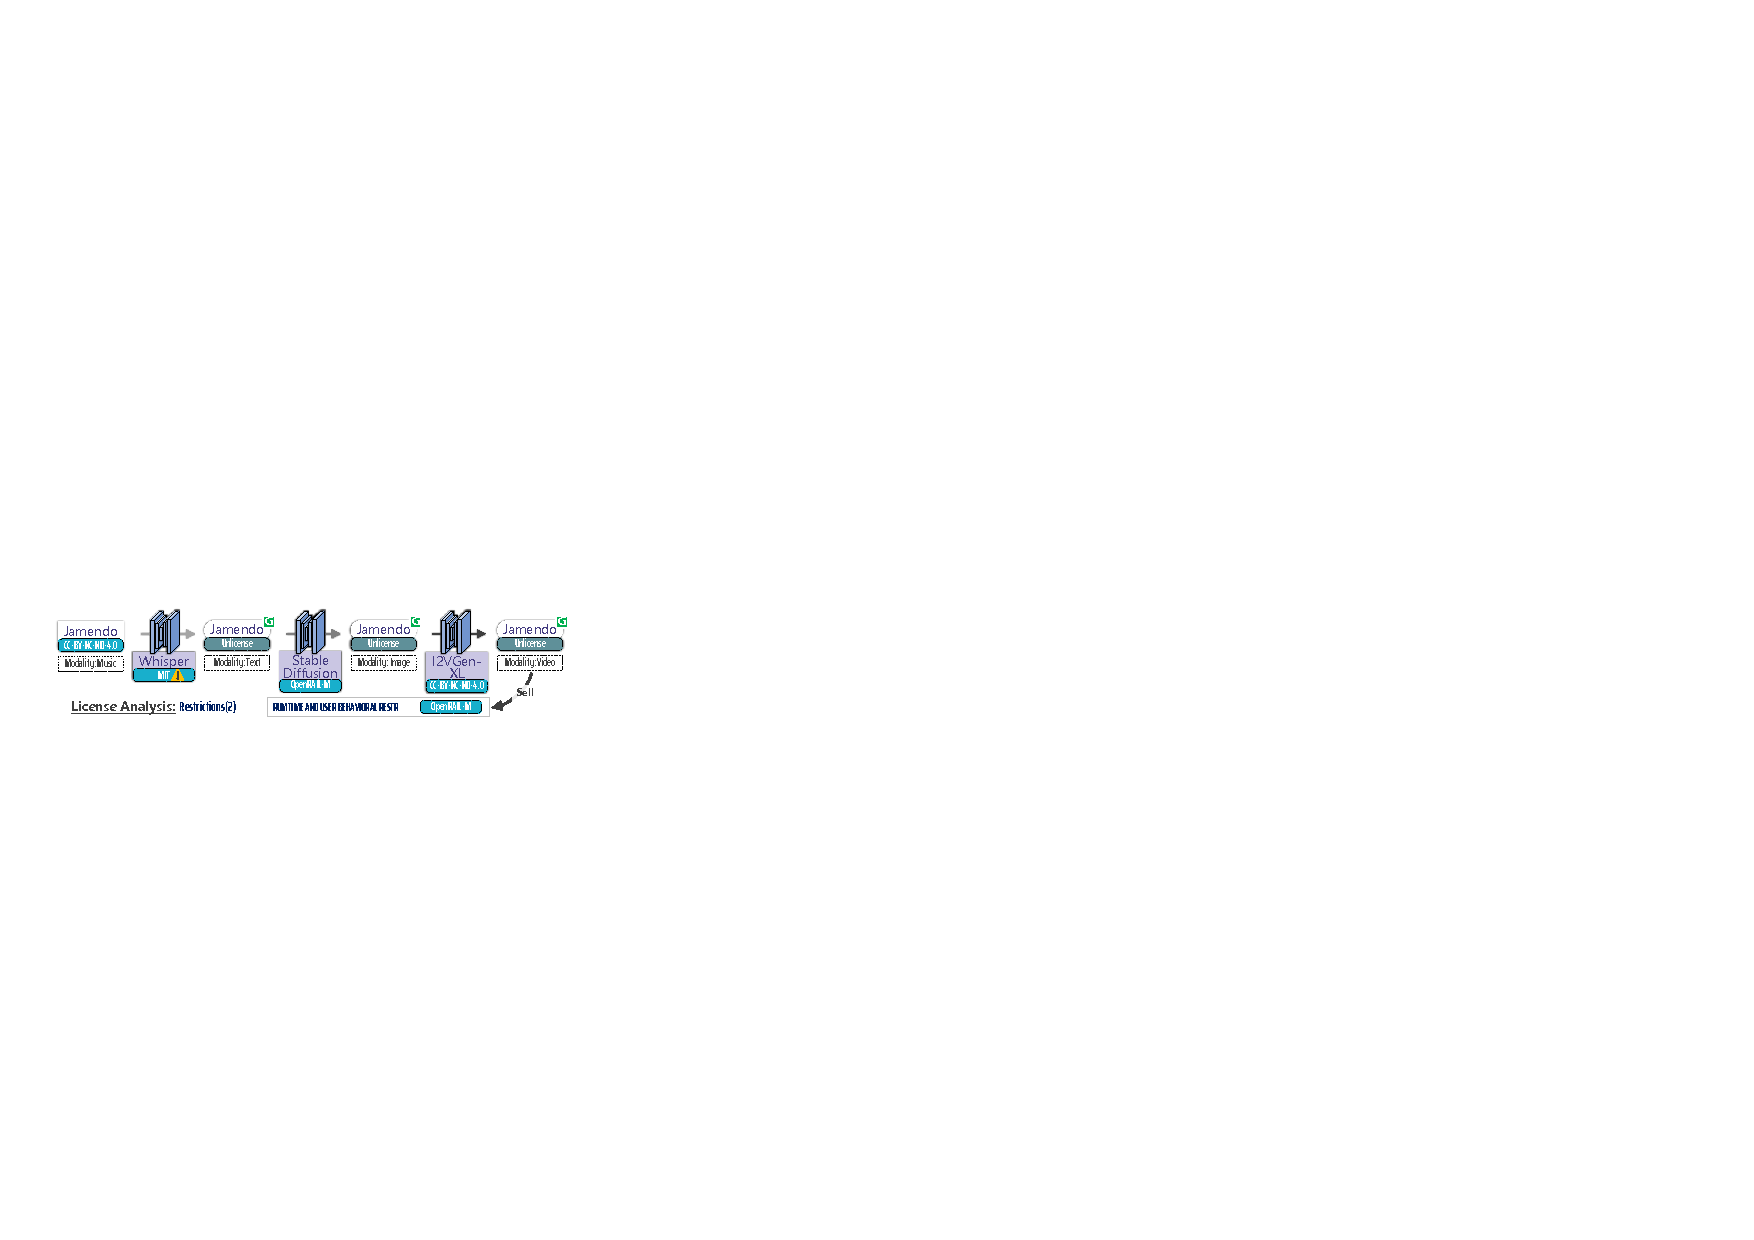
\includegraphics[width=\linewidth]{fig/case3.pdf}
    \caption{Case Study \Romannum{3}: Pipeline.}
    \Description{}
    \label{fig:case3}
\end{figure}

\begin{figure}[t]
    \centering
    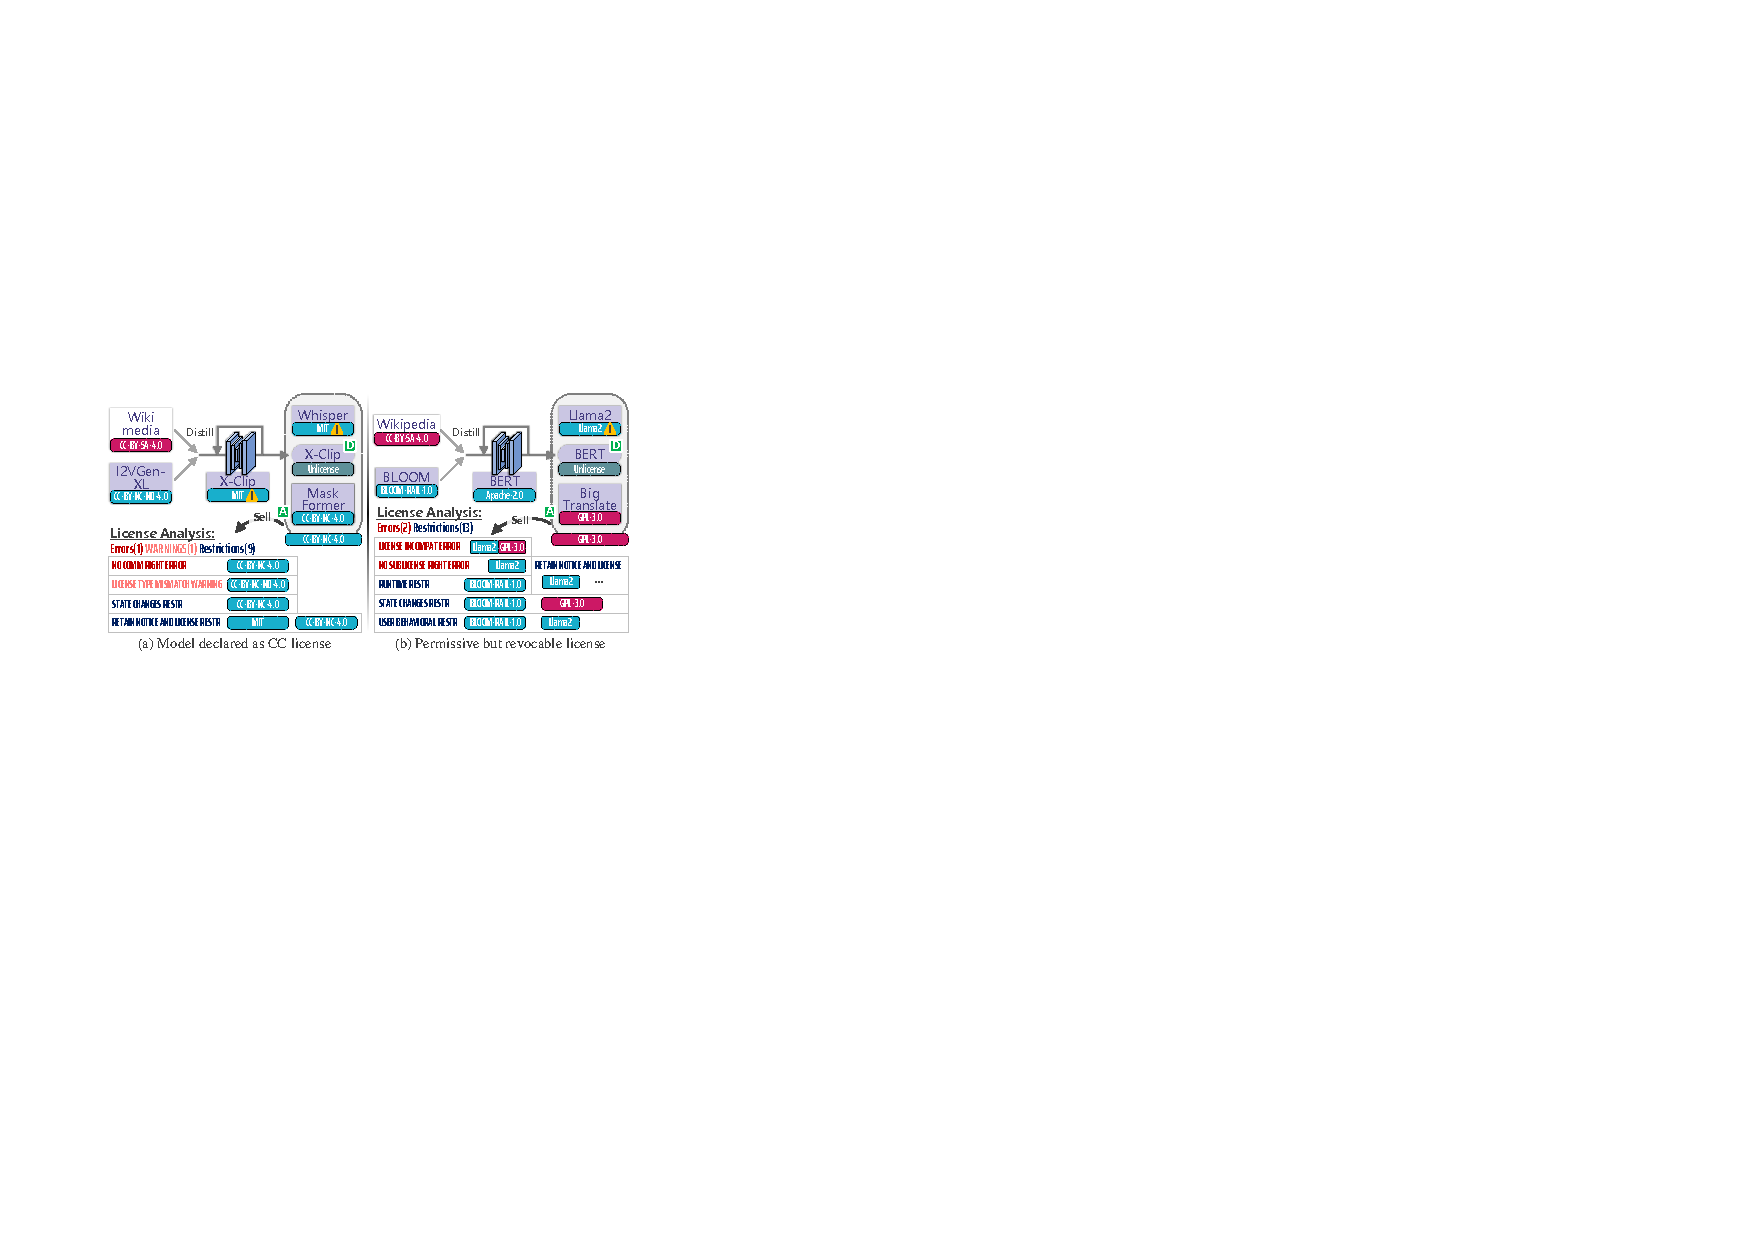
\includegraphics[width=\linewidth]{fig/case4.pdf}
    \caption{Case Study \Romannum{4}: distillation and model averaging.}
    \Description{}
    \label{fig:case4}
\end{figure}

\begin{figure}[t]
    \centering
    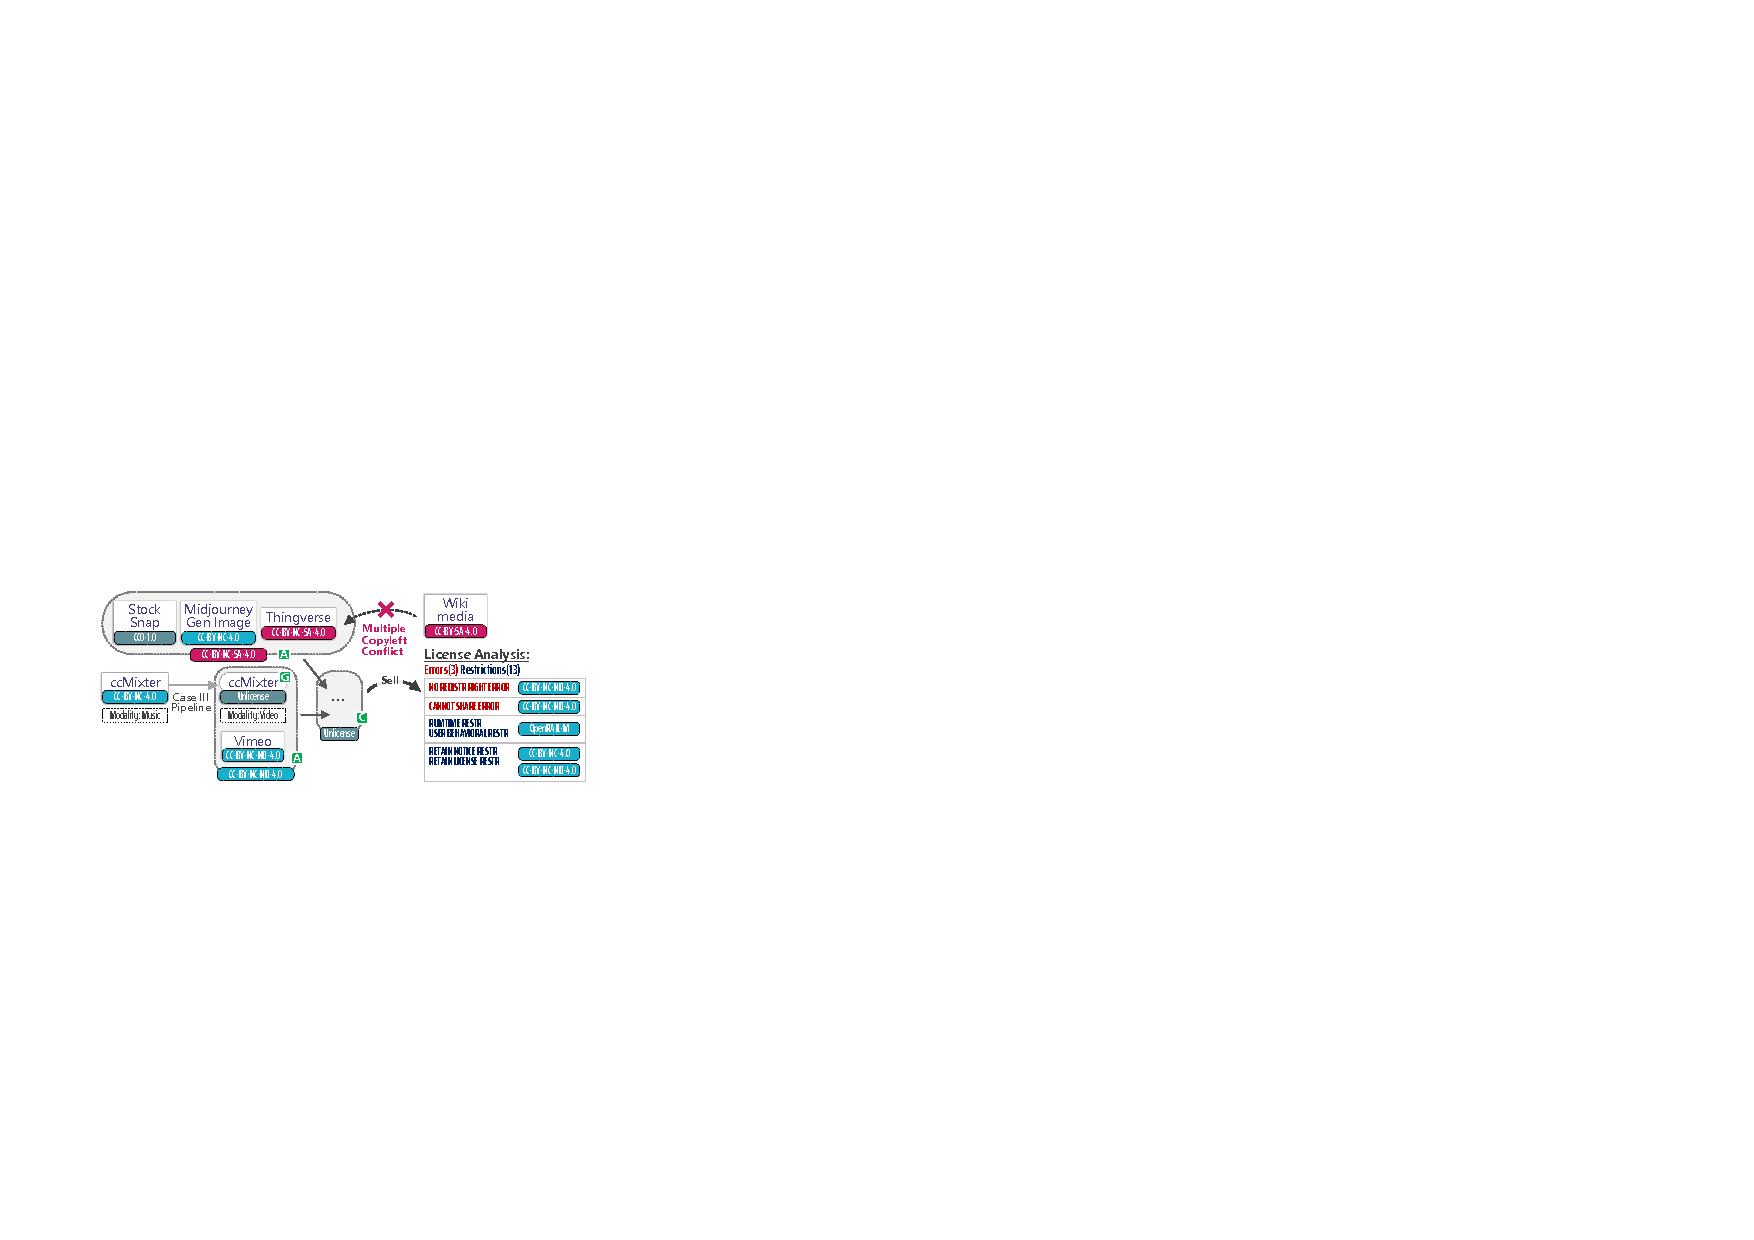
\includegraphics[width=\linewidth]{fig/case5.pdf}
    \caption{Case Study \Romannum{5}: distillation and model averaging.}
    \Description{}
    \label{fig:case5}
\end{figure}